O HSM é composto de duas estruturas com saliências, o rotor e o estator, seu circuito magnético é excitado pela combinação de espiras e magnetismo permanente, imã. As espiras são montadas nos polos do estator e o imã no rotor. Como mostrado na Figura \ref{fig:estrutura_HSM}. \cite{SteppingBook}

	\begin{figure}[!h]
		\centering
		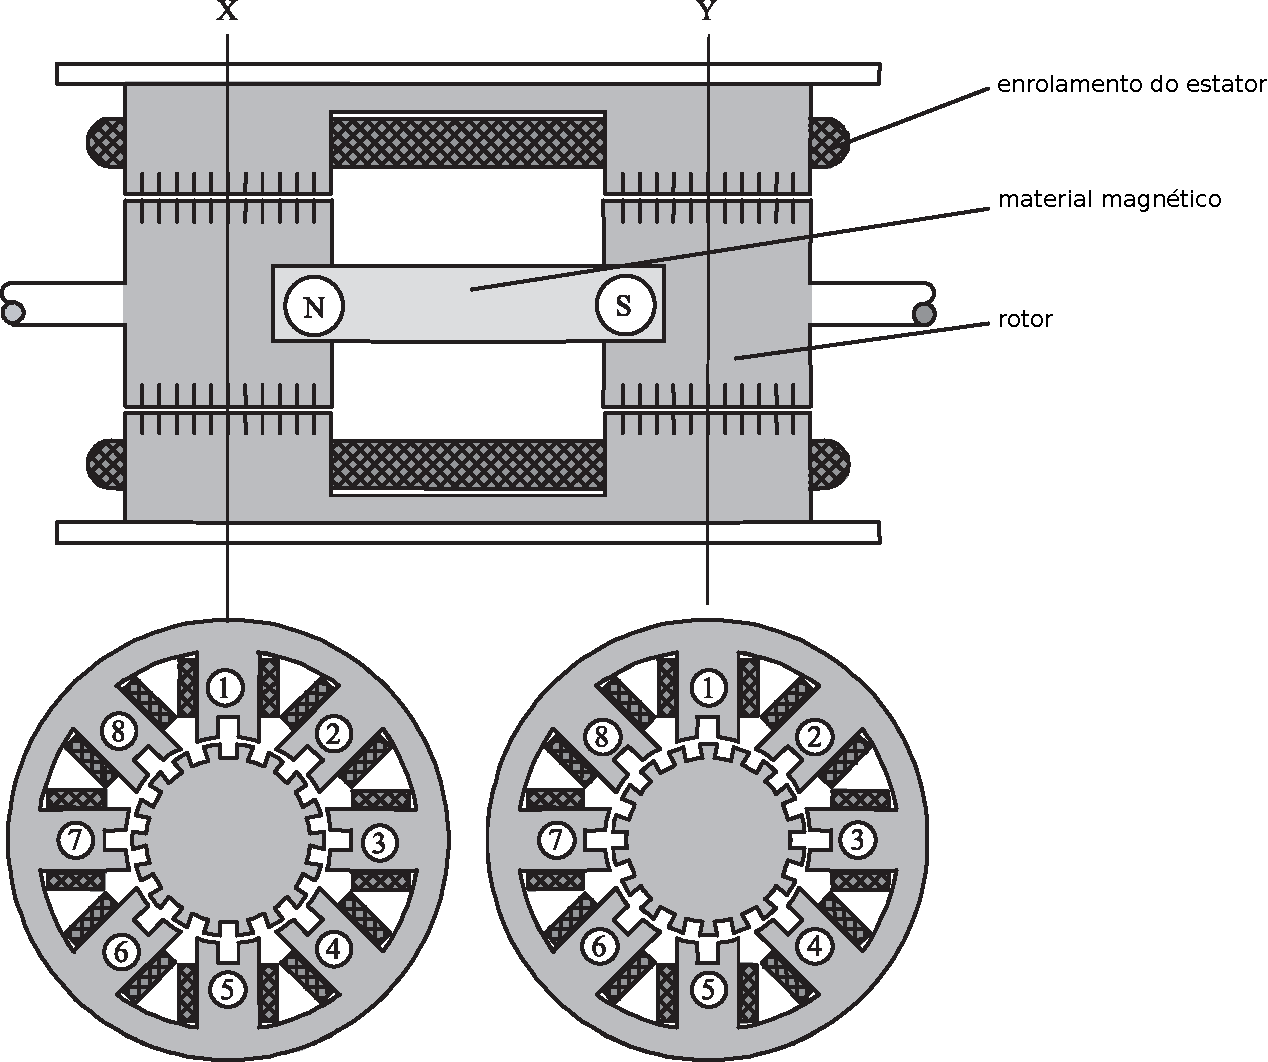
\includegraphics[width = \columnwidth]{Images/estrutura_HSM.pdf}
		\caption{Visão de lado e de frente do HSM. \cite{SteppingBook}}
		\label{fig:estrutura_HSM}
	\end{figure}
	
Tipicamento o motor de passo híbrido tem oito polos no estator e em cada polo tem entre dois a seis dentes, ou também chamado \emph{teeth}, do inglês. Ele tem ainda comumente um pequeno largura de passo, tipicamente 1,8º. \cite{SteppingBook}

As principais partes constituintes de um HSM comercial é mostrado na Figura \ref{fig:partes_SM}.

	\begin{figure}[!h]
		\centering
		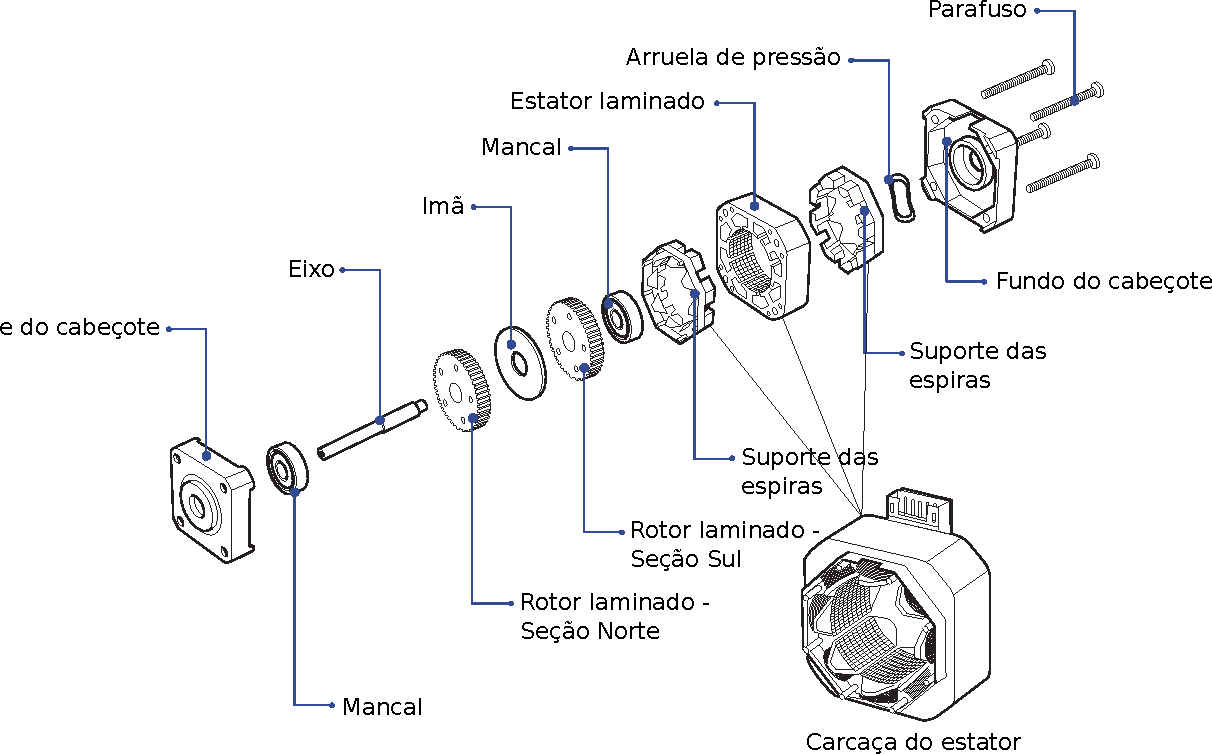
\includegraphics[width = \columnwidth]{Images/partes_HSM.pdf}
		\caption{Partes constituintes de um HSM comercial. \cite{MoonsHSM}}
		\label{fig:partes_SM}
	\end{figure}